\section{Preliminary work}
\label{sec:preliminary_work}
The HAP project was initiated in 2017 by PIs RR and YNY.
The lead author on our first paper (\cite{Fu2018_SIAM}) was Szu-Pei Fu,
who was PI YNS's PhD student and is currently a postdoc with PI RR.
The collaboration involved theoretical work and simulation. The theoretical
work included model development, proving the first variation formula
\eqref{stress} and force-free law, and an energy-based  uniqueness
theorem for the exterior domain problem \eqref{SL}.
Coauthors Andreas Kl\"ockner (Computer Science, UIUC, NSF CAREER \#1654756)
and his PhD student Matt Wala provided their Quadrature by Expansion, or QBX
algorithm and Fu ran simulations on NJIT clusters.   

The simulation results were encouraging. The small particle-number
simulations successfully demonstrated gradient-driven self-assembly of amphiphilic
particles into two-dimensional micelles, bilayer membranes. The model parameters
where the decay length $\rho$, interfacial tension $\gamma$, particle geometry, and
repulsion strength. The particle diamaters were set equal to monolayer thickness, 
2.0 nm \cite{Boal}, and we chose a repulsion strength that gave adequate interparticle 
spacing. For the decay length, we used $\rho = 2.5$ nm based on measurements of hydrophobic
attraction between surfactant-coated \cite{Eriksson1989,Lin2005,Parsegian,Israelachvili80}.
For the interfacial tension, we used $\gamma = 4$ pN nm$^{-1}$
based on measurements for single-component bilayer lipid membranes
\cite{GarciaSaez, KUZMIN2005, Petelska2012, Jackson2016}.

\begin{wraptable}[10]{r}{0.55\textwidth}
\begin{center}
  \begin{tabular}{|l|r|r|p{0.1\textwidth}|}
    \hline
          & HAP                     & exper. value          & ref.\\
    \hline 
    $\KB$ & $11 \pm 2.5$ \kBT       & 10 \kBT               & \cite{Naetal15,VeBrPa15,NAGLE2000159,PhysRevLett.113.248102}\\
    \hline 
    $\KA$ & $34$ \kBT \; nm$^{-2}$  & 30--40 \kBT nm$^{-2}$ & \cite{Nagle17, Nagle17-2}\\
    \hline 
    $\KTH$ & $12$ \kBT \; nm$^{-2}$ & 10 \kBT nm$^{-2}$     & \cite{KUZMIN2005, KoNa15} \\ \hline
  \end{tabular}
\end{center}
\caption{\label{tab:moduli} \footnotesize Comparision of values elastic
  moduli from the experimental literature and values derived by HAP
  simulation.} 
\end{wraptable}
We performed three types of simulations. The first measured bending by loading
a planar bilayer. The second used a harmonic bond to dilate a circular bilayer.
The third measured tilt using a decay equation from  \cite{KUZMIN2005}.
These simulations isolated the deformations of \eqref{ansatz3}, enabling
us to read off elastic moduli from simulation data. The results agreed remarkably 
well with the values reported in the experimental literature, 
Table~\ref{tab:moduli}. The agreement is underscored by the fact
that the two, main HAP parameters $\gamma$ and $\rho$ were assigned
physical values from the outset, rather than being tuned. 

The PIs BQ, RR, YNY and Peter Fu initiated a collaboration in summer, 2020. 
The present proposal is the outgrowth of this collaboration. We have created
a compact numerical solver and included background flow in the simulations. 
%%%%%%%%%%%%%%%%%%%%%%%%%%%%%For Specific Aim 3
%The background flow enters by replacing the third equation in \eqref{eq:stokes} 
%with the condition $(\mathbf{u} -\mathbf{u}_{\infty})(\mathbf{x}) 
%\to \mathbf{0}$ as $|\mathbf{x}| \to \infty$. To incorporate the far-field flow, 
%and using the representation 
%\begin{align}
%\label{PowerMiranda}
%  {\bf u} = {\bf u}_{\infty} + K\boldsymbol{\eta} + 
%    \sum_{i=1}^N S(\cdot, {\bf a}_i) {\bf F}_i + 
%                 R(\cdot, {\bf a}_i) {\bf G}_i.
%\end{align}
%The symbols $S$ and $R$ are Stokeslets and rotlets supported at the respective
%particle centers \cite{leal_2007} and $K\boldsymbol{eta}$ is a layer potential for the
%unknown density function $\boldsymbol{\eta}.$ The
%representation~\eqref{PowerMiranda} automatically satisfies all
%equations, with the exception of the rigid motion conditions. The rigid
%motion conditions follow by requiring the viscous stress vanishes across
%the particle boundaries.

%\begin{wrapfigure}[13]{l}{0.30\textwidth}
%\centerline{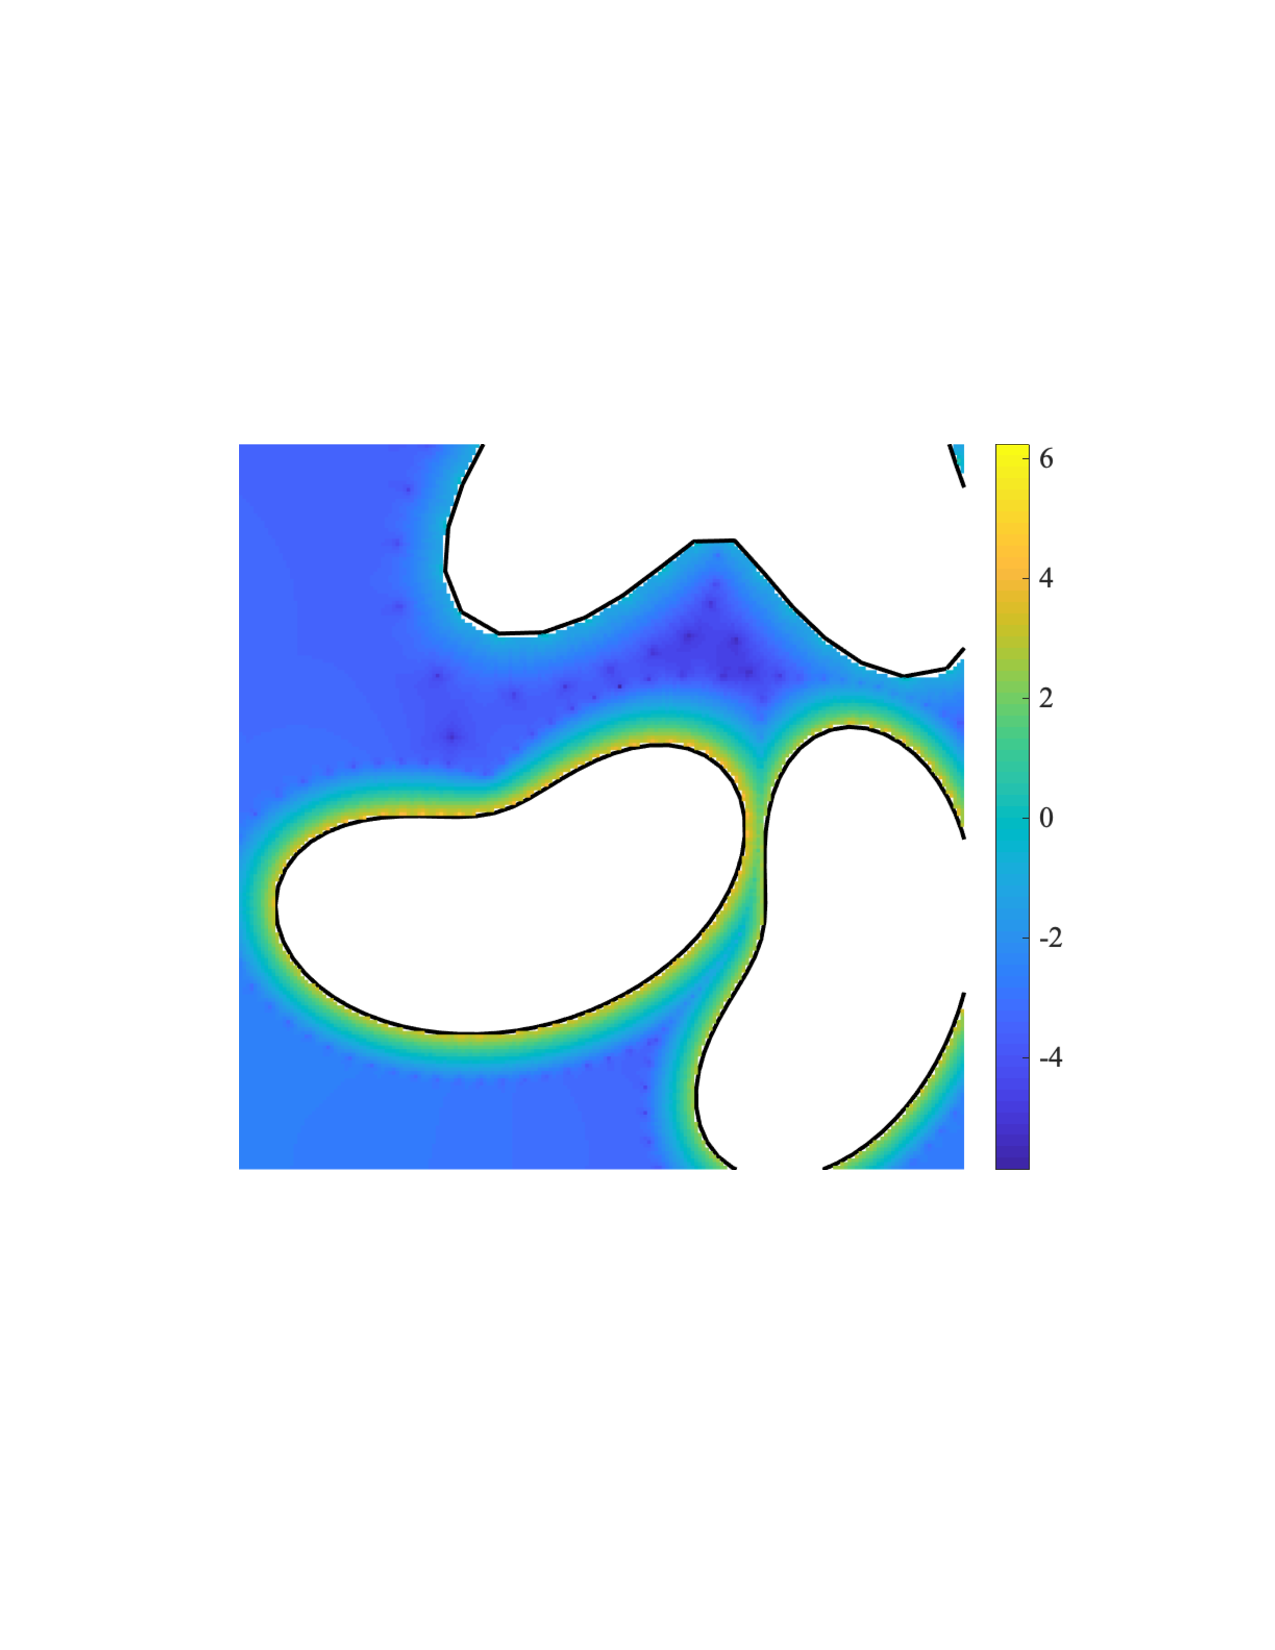
\includegraphics[width=0.30\textwidth]{figures/BIError.pdf}}
%  \vspace{-8pt}
%\caption{
%\label{fig:bierror}  
%\footnotesize The false color map shows how numerical quadrature of
%  layer potentials loses accuracy near the particle boundaries.  The
%  color bar is for $\log_{10}.$}
%\end{wrapfigure}
%\textbf{Novel reciprocal identities.} 
%The force and torque formulas~\eqref{forceandtorque} require the
%hydrophobic stress along the particle boundaries. Unfortunately,
%standard quadrature formulas to estimate $\nabla u$ on the particle
%boundaries introduces large amounts of quadrature error
%(Figure~\ref{fig:bierror}). Therefore, it is useful to devise reciprocal
%identities for the force and torque on body $i$ that does not
%require integration along body $i$. One identity, that we have proved,
%is
%\begin{align}
%    \label{eq:reciprocal}
%{\bf F}_{\text{hydro},i} = \sum_{j \neq i} \int_{\partial P_i}
%[\boldsymbol{\sigma}_{ij} + \boldsymbol{\sigma}_{ji}]\boldsymbol{\nu}\,\dif S,\quad
%{\bf G}_{\text{hydro},i} = \sum_{j \neq i} \int_{\partial P_i} ({\bf
%  x}-\mathbf{a}_i) \times [\boldsymbol{\sigma}_{ij} +
%  \boldsymbol{\sigma}_{ji}]\boldsymbol{\nu}\,\dif S, 
%\end{align}
%for $i=1,\ldots,N$. Here, $u_i$ is the solution of the screened Laplace
%equation when only the contribution from particle $i$ is considered and
%$\boldsymbol{\sigma}_{ij} = \rho^{-1} u_iu_j {\bf I} + \rho(\nabla u_i
%\cdot \nabla u_j {\bf I} - 2 \nabla u_i \otimes \nabla u_j)$.
%Because of the double layer potential jump relations, \eqref{eq:reciprocal} 
%does not require knowledge of $\nabla u$ on the particle boundary, and this
%is enormously beneficial for calculating force and torque.

\subsubsection{Two-dimensional vesicles in shear flow}
We have simulated two-dimensional vesicles in the background shear flow
$\mathbf{u}_{\infty} = \dot{\gamma} x_2 \mathbf{i}_1$. The numerical solver
is written in the Matlab language runs on a desktop without parallelization. 
The initially circular vesicle bilayers rotate and elongate with the shear flow, 
and approach a steadily tank-treading ellipse.

There are a number of well-established mathematical models of vesicles
in shear flow \cite{torres-sanchez_millan_arroyo_2019, mahapatra_saintillan_rangamani_2020, 
Steigmann99, C6SM02452A}. We are trying to assess which constituative
assumption the particle-based bilayer satisfies. 
Our preliminary results show that the particle-based bilayers have the same
large area modulus as real lipid bilayer membranes, so we expect
realistic results from our flow simulations. Under moderate shear rates,
the vesicle elongates and takes on the tank-treading elliptical shape.
We can directly check for area compressibility conservation properties
from the particle simulation by tracking the change in area density of
the midplane as a function of shear flow rate, along with evaluating the
tangential divergence of the velocity.

Bilayer membranes have a small permeability to water
\cite{323e9a2f0c58487ea82518d7a1f96485}, and modelers often assume a
vesicle membrane that conserves volume. In our particle-based approach,
water motion across the bilayer is limited by the size of the gaps
between the particles, which is an artifact of coarse-graining.  Making
these gaps smaller comes at the expense of numerical accuracy, and we
will assess if there is a reasonable trade-off between approximate
volume conservation and simulation complexity. 

Finally, the particle-based vesicle bilayers have two distinct leaflets
consisting of the particles in contact with the vesicle interior, and
those in contact with the surrounding fluid. Since there is a nonzero
separation between these layers, an important effect we observe is that
the leaflets slide against one another under shear flow.  This implies
that part of the viscous dissipation in the aqueous phase is enhanced by
intermonolayer friction~\cite{SHKULIPA2005823, ShkulipaThesis}.
Intermonolayer slip enters zero-thickness membrane models as a velocity
jump boundary condition and leads to multiple solution
states~\cite{schwalbe_vlahovska_miksis_2010}.  In the present proposal,
intermonolayer slip is an artifact of monolayer independence  and we can
control for slip as a function of shear rate, vesicle diameter, and
particle geometry.



%\subsection{Two-dimensional vesicle hydrodynamics in shear flow} 
%The motion of vesicles in shear flow is an important problem in the
%applied mathematics because simulations can reveal mechanical
%properties of membranes and lead to an enhanced understanding of
%deformable particle laden flows \cite{Sinha15}. 
%
%
%\begin{wrapfigure}[10]{r}{0.2\textwidth}
%\centerline{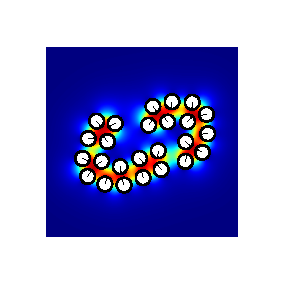
\includegraphics[width=0.2\textwidth]{figures/PW_fig5.pdf}}
%\vspace{-8pt}
%\caption{\label{fig:rupture} \footnotesize Rupture of tank-treading vesicle under strong shear flow.}
%\end{wrapfigure}
%
%To implement a vesicle in shear flow in the context of hydrophobic
%potentials and mobility problem, we consider a shear flow in the
%far-field $\mathbf{u}_{\infty} = Uy\mathbf{i}_x$ in the direction of the
%$x$-axis (Figure \ref{fig:tanktreading}A). As illustrated in Figure
%\ref{fig:tanktreading}, the particle based approach supports
%inter-leaflet slip, and this can be used to determine inter-leaflet and
%in-plane shear viscosities. 
%
%This field satisfies the linear Stokes system but does not give rise to a rigid motion at the particle interfaces. 
%To have a rigid motion, we change variables $\mathbf{u} = \tilde{\mathbf{u}}+ \mathbf{u}_{\infty}$ and 
%for the new field $\tilde{\mathbf{u}}$ vanishing at infinity we let 
%$\tilde{\mathbf{u}}|_{\partial P_i} = \mathbf{v}_i + \boldsymbol{\omega}_i \times (\mathbf{x} - \mathbf{a}_i)$ 
%where $(\mathbf{v}_i,\boldsymbol{\omega}_i)$ are the unknown translation and angular velocities of the 
%$i$th particle $P_i.$  
%
%\begin{wrapfigure}[17]{l}{0.4\textwidth}
%\centerline{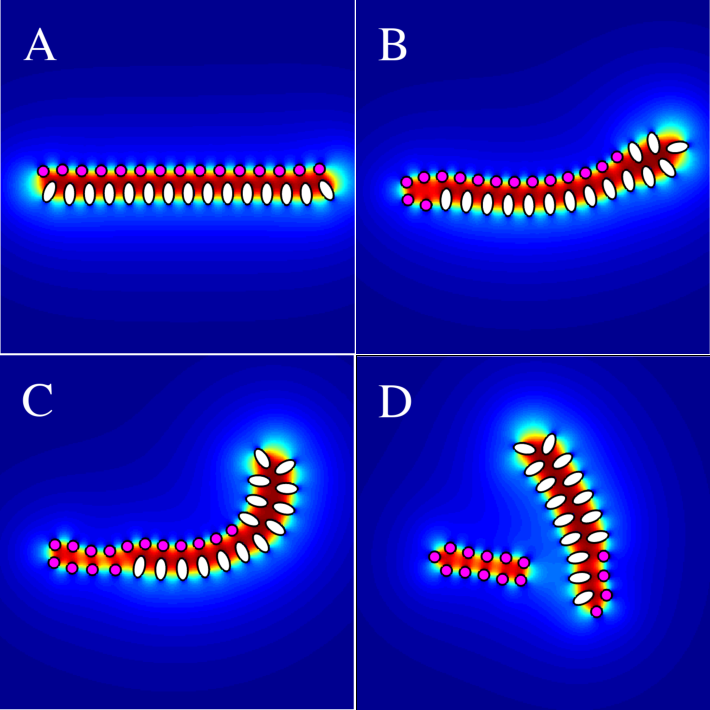
\includegraphics[width=0.4\textwidth]{figures/PW_fig2.pdf}}
%\caption{\label{fig:demixing} An initial assembly of small and 
%large particles spontaneous segregates into two smaller bodies. }
%\end{wrapfigure}
%The HAP simulations show vesicle tank-treading. Under the external shear flow, the initially circular 
%vesicle rotates in the clockwise direction. As the rate of rotation increases, the vesicle approaches
%a steadily tank-treading ellipse. In Figure \ref{fig:tanktreading}B-D, the solid curves are ellipses fit to the particle centers
%and midplane respectively. In the non-dimensionalized system, the particles have diameter 2, on the order of $\rho,$ 
%and the vesicle diameter is about 14. 
%\todo[inline]{missing units. nm?}
%Figure~\ref{fig:tanktreading}E shows the aspect ratio of the major to minor axes reaching an equilibrium value in the 
%red and blue curves, yet oscillating in the high-shear rate (yellow) curve.
%The tank-treading vesicle elongates and becomes more horizontal 
%with an increase in flow rate or 
%with a decrease in stiffness (effected by decreasing $\rho = 4$ to $\rho = 2$). 


%For large shear flow rates, there is an increase in arc length. Here arc
%length refers to the the mid-plane circumference. Thus, some of the
%external force is going into stretching the vesicle---the other part is
%going into bending and viscous dissipation. From our experiments, we
%find that the vesicle ruptures once stretching exceeds about 5 \% (see
%Figure \ref{fig:rupture}). Finally, movies of the tank-treading motion
%show a slip velocity between the outer and inner leaflets Figure
%\ref{fig:tanktreading}G. We have illustrated this by tracking the
%distance between two reference particles in the inner and outer leaflet
%(Figure \ref{fig:tanktreading}B \& D, green and blue particles). With
%moderate shear rates or greater adhesion, the particle pair moves in
%tandem (in Figure \ref{fig:tanktreading}H, blue and red curves, their
%distance is more or less constant). For a large shear rate, the
%particle separates as the two leaflets slide against one another. 

%\begin{figure}
%\begin{center}
%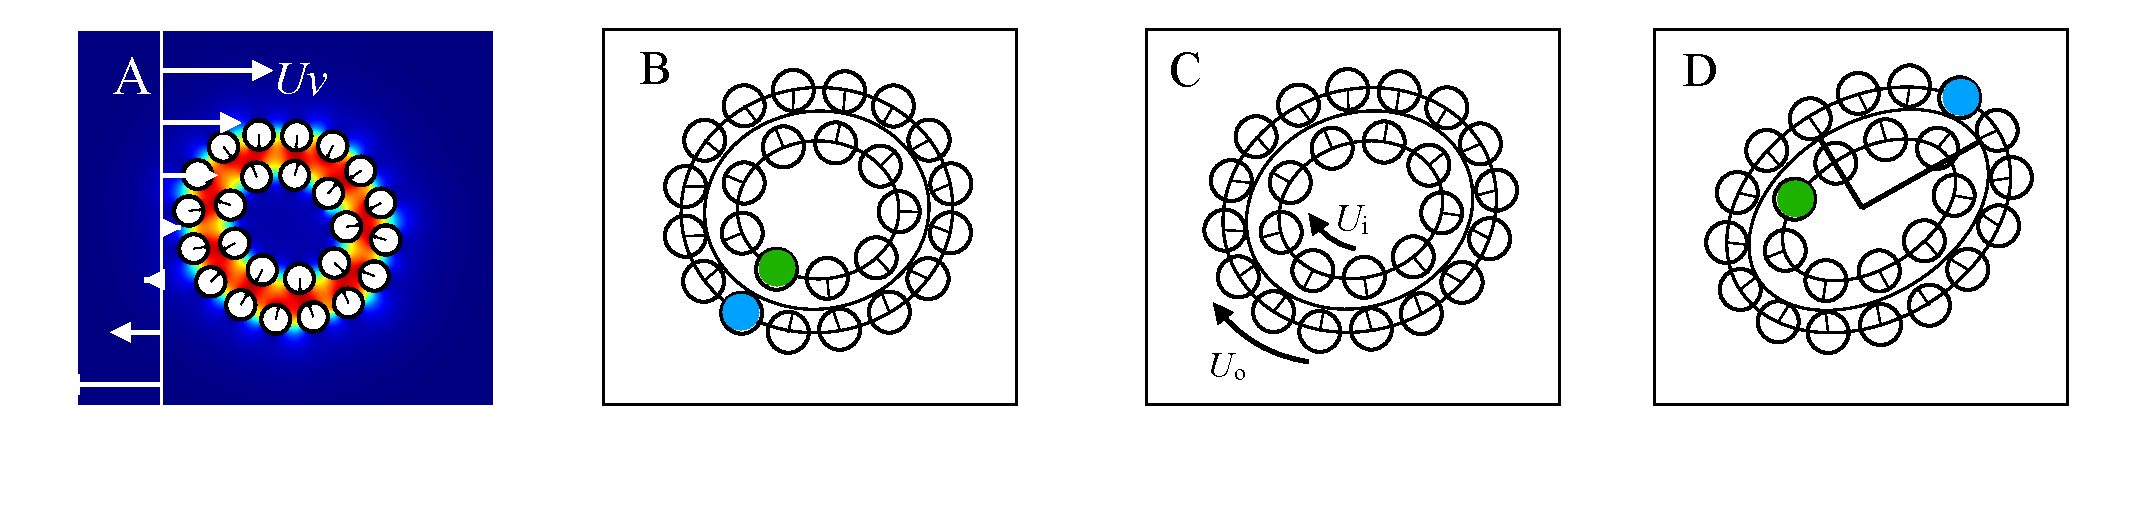
\includegraphics[width=1\textwidth]{figures/PW_fig1A-D.pdf}
%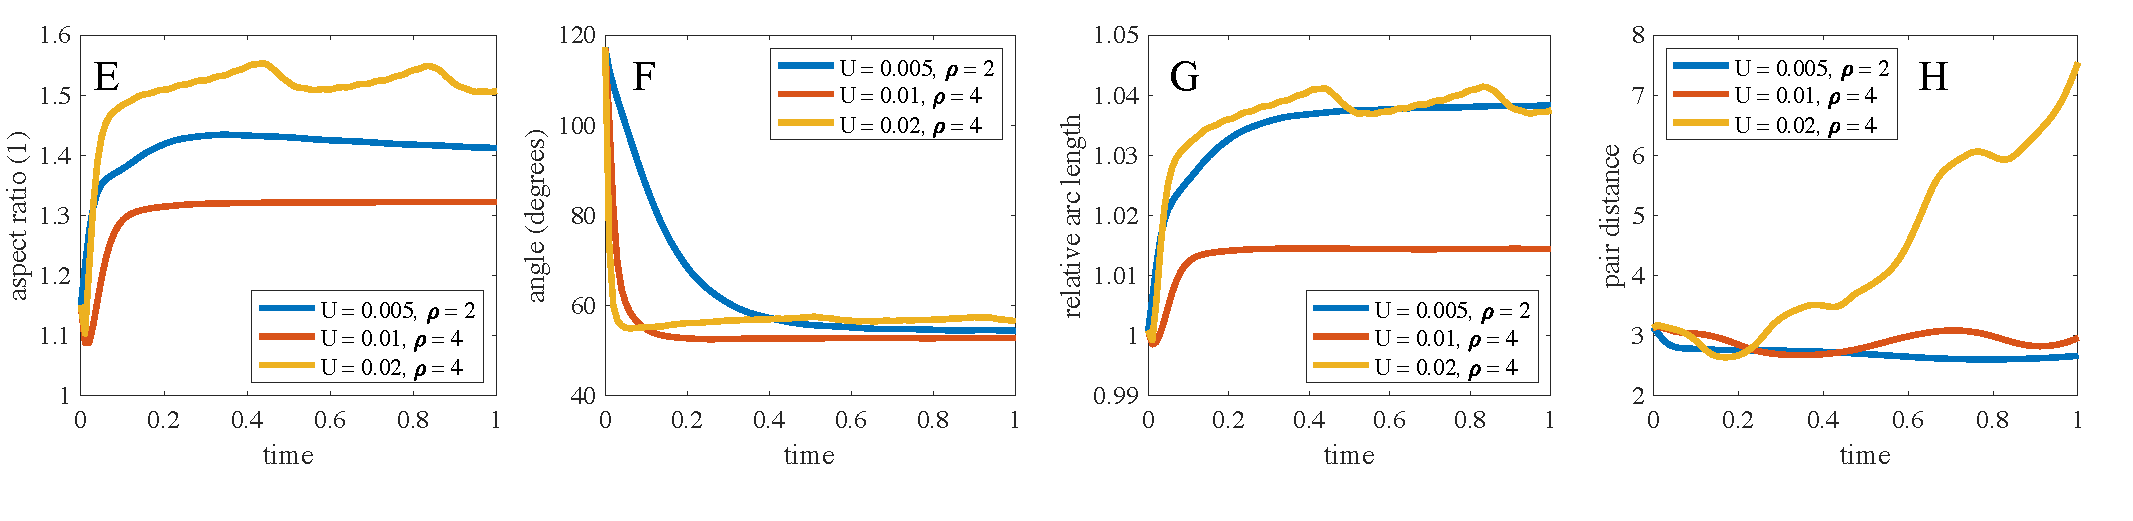
\includegraphics[width=1\textwidth]{figures/PW_fig1E-H.pdf}
%\end{center}
%\vspace{-0.3in}
%\caption{\label{fig:tanktreading}\footnotesize (A) A vesicle formed by
%  amphiphilic particles in shear flow, and the tank-treading motion
%  (B)--(D). The separation of particle pairs in (B) and (C) illustrate
%  inter-leaflet slip.  (E)--(G) Tank-treading reaches a steady state in
%  elliptical aspect ratio, major-axis angle, and circumference.}
%\end{figure}


%\begin{wrapfigure}[12]{r}{0.2\textwidth}
%\centerline{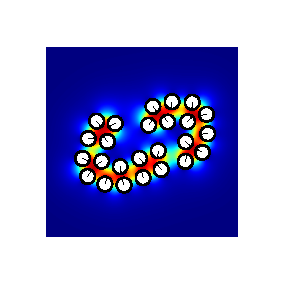
\includegraphics[width=0.2\textwidth]{figures/PW_fig5.pdf}}
%\caption{\label{fig:rupture} Rupture of tank-treading vesicle under strong shear flow.}
%\end{wrapfigure}
%




